%%%%%%%%%%%%%%%%%%%%%%%%%%%%%%%%%%%%%%%%%%%%%%%%%%%%%%%%%%%%%%%%%%%%%%
%
% Institut für Information Systems Engineering
% Forschungsgruppe INSO
% Arbeitsgruppe ESSE
% https://establishing-security.at/
% lva.security@inso-world.com
%
%%%%%%%%%%%%%%%%%%%%%%%%%%%%%%%%%%%%%%%%%%%%%%%%%%%%%%%%%%%%%%%%%%%%%%

\documentclass[12pt, a4paper, titlepage, oneside]{scrartcl}
\newcommand{\lang}{de}
\usepackage{esseProtocol}

%%%%%%%%%%%%%%%%%%%%%%%%%%%%%%%%%%%%%%%%%%%%%%%%%%%%%%%%%%%%%%%%%%%%%%
%
% FOR STUDENTS
%
%%%%%%%%%%%%%%%%%%%%%%%%%%%%%%%%%%%%%%%%%%%%%%%%%%%%%%%%%%%%%%%%%%%%%%

% Team number or "0" for Lab0
%TODO team number
\newcommand{\team}{44}
% Date
%TODO fill in creation date
\newcommand{\datum}{\today}
%TODO lab number
% valid values: "Lab0", "Lab1" (be sure to use Uppercase for first character)
\newcommand{\lab}{Lab1}

%TODO name of course
\newcommand{\lvaname}{Einführung in Security} % if 6 ECTS variant, otherwise: Introduction to Security
%TODO number of course
\newcommand{\lvanr}{194.157} % if 6 ECTS variant, otherwise: 183.594
%TODO year and term, for example: "2024 S" or "2024 W", etc.
\newcommand{\semester}{2024 W}

% Student data in Lab0 or 1. student of team in Lab1
\newcommand{\studentAName}{Kevin Csele}
\renewcommand{\studentAMatrnr}{12122544}

% 2. student of team in Lab1, for Lab0 or if your team has less students, remove these 2 lines
\newcommand{\studentBName}{Clemens Schneider}
\renewcommand{\studentBMatrnr}{12219440}

% 3. student of team in Lab1, for Lab0 or if your team has less students, remove these 2 lines
\newcommand{\studentCName}{Luka Twaroch}
\renewcommand{\studentCMatrnr}{12226627}

% 4. student of team in Lab1, for Lab0 or if your team has less students, remove these 2 lines
\newcommand{\studentDName}{Wen Long Zhou}
\renewcommand{\studentDMatrnr}{12225657}

% 5. student of team in Lab1, for Lab0 or if your team has less students, remove these 2 lines
\newcommand{\studentEName}{Ramin Shaikh}
\renewcommand{\studentEMatrnr}{12123657}

%%%%%%%%%%%%%%%%%%%%%%%%%%%%%%%%%%%%%%%%%%%%%%%%%%%%%%%%%%%%%%%%%%%%%%
%
% DO NOT CHANGE THE FOLLOWING PART
%
%%%%%%%%%%%%%%%%%%%%%%%%%%%%%%%%%%%%%%%%%%%%%%%%%%%%%%%%%%%%%%%%%%%%%%

\newcommand{\colormode}{color}
\newcommand{\dokumenttyp}{Abgabedokument \lab}

\begin{document}
	\maketitle
	\setcounter{section}{0}
	\setcounter{tocdepth}{2}
	\tableofcontents

	%%%%%%%%%%%%%%%%%%%%%%%%%%%%%%%%%%%%%%%%%%%%%%%%%%%%%%%%%%%%%%%%%%%%%%
	%
	% CONTENT OF DOCUMENT STARTS HERE
	%
	%%%%%%%%%%%%%%%%%%%%%%%%%%%%%%%%%%%%%%%%%%%%%%%%%%%%%%%%%%%%%%%%%%%%%%
	\newpage

	\section{Der Service war auch schon besser ...}

	\subsection{Achtung! Streng geheim!}
	Um diese Aufgabe zu l\"osen, hat es gen\"ugt, das besagte PDF im Browser zu \"offnen.
	Der ``streng geheime`` String befand sich im Titel des Tabs.

	\subsection{Eine schräge Nummer}
	Die Rechnungsnummer wurde zwar von einem schwarzen Rechteck verdeckt, ließ sich
	jedoch ganz einfach kopieren, indem man die betroffene Stelle markiert -> Strg
	+ C

	\subsection{Was letzte Preis?}
	Selbes Spiel, auch der Preis ließ sich ganz simpel herauskopieren.

	\subsection{IBANs sollte man verbannen!}
	Um den IBAN aufzudecken, habe ich PDF-XChange verwendet, um das schwarze Rechteck
	mit dem Objektbearbeitungswerkzeug zu entfernen.

	\section{Wireless Time Travel}

	\subsection{Vier zukunftssichere Handschl\"age}
	Nicht gelöst.

	\subsection{Code der Zukunft}
	Nicht gelöst.

	\subsection{Ungew\"ohnlich verschl\"usselte Botschaft}
	Nicht gelöst.

	\subsection{Geheimnisvoller Zugang: superboss}
	Nicht gelöst.

	\subsection{Unbrauchbarer Schl\"ussel}
	Nicht gelöst.

	\subsection{Einen Schl\"ussel f\"ur einen Schl\"ussel! Echt jetzt?!}
	Nicht gelöst.

	\subsection{Verborgenes Protokoll}
	Nicht gelöst.

	\section{Bot Bot Bot Bot}

	\subsection{I keep you my little secret ...}
	Nicht gelöst.

	\section{C\"asars Schl\"usselbund}

	\subsection{Schl\"ussel. Knacken.}
	Nicht gelöst.

	\subsection{Passw\"orter Retten.}
	Nicht gelöst.

	\section{Paranoider Mozart}

	\subsection{MozART.}
	Nicht gelöst.

	\newpage

	\section{Zertifiziertes Durcheinander}

	\subsection{Zertifizieren ist schwer}
	Um den Certificate Signing Request zu erstellen habe ich den folgenden Befehl
	verwendet: \lstinline{openssl req -newkey rsa:4096 -sha512 -config openssl.cnf -out csr.csr -subj "/CN=12123657-Intermediate-CA-WS2024/OU=ESSE-Lab1-Exercise"}
	\begin{itemize}
		\item \lstinline{req} ist der Befehl um einen CSR zu erstellen
		\item \lstinline{-newkey rsa:4096} spezifiziert, dass ein neuer Key (4096-Bit RSA) erstellt werden soll
		\item \lstinline{-sha512} gibt an, dass sha512WithRSAEncription als Signaturalgorithmus verwendet werden soll
		\item mit \lstinline{-config} wird angegeben, welches config file zu verwenden ist
		\item \lstinline{-out} bestimmt das output-file und
		\item \lstinline{-subj "/CN=12123657-Intermediate-CA-WS2024/OU=ESSE-Lab1-Exercise"} definiert die gewünschten Namens-Parameter im CSR.
	\end{itemize}
	Das config file dient dazu, die nötigen X509v3 Parameter zu setzen und sieht aus wie folgt:
	\begin{lstlisting}[caption=openssl.cnf,label=code:opensslConfig,style=simple]
		[ req ]
		default_bits           = 4096
		default_md             = sha512
		default_keyfile        = privkey.pem
		distinguished_name     = req_distinguished_name
		req_extensions          = v3_req

		[ req_distinguished_name ]

		[ v3_req ]
		subjectKeyIdentifier = hash
		basicConstraints = critical, CA:true, pathlen:0
		keyUsage = critical, Certificate Sign, CRL Sign
	\end{lstlisting}
	Nach Ausführung des oben genannten Befehls, wird der CSR in der Datei csr.csr gespeichert,
	diese wurde im Abgabetool eingereicht.

	\section{Zeitreise durch das World Wide Web}

	\subsection{Wieder Elvis}
	Nicht gelöst.

	\subsection{C\"asarMussWeg! MussC\"asarWeg?}
	Nicht gelöst.

	\subsection{dackboor.}
	Nicht gelöst.

	\subsection{Schlechtes Timing (Time Travel Edition)}
	Nicht gelöst.

	\subsection{Sorcerer ... ?}
	Nicht gelöst.

	\newpage

	\section{Seitlich fließend}

	\subsection{Newton und Co KG.}
	Bei dieser Aufgabe war es gefragt, sich über nc mit einem Server zu verbinden und eine Flag zu finden.
	Anfangs bin ich wie folgt vorgegangen:
	\begin{itemize}
		\item Verbinden mit dem Server über tese: 
		\begin{itemize}
			\item \lstinline{ssh lab} (lab ist die gespeicherte ssh Konfiguration für tese)
			\item \lstinline{nc 10.10.10.202 7044} (IP und Port laut Angabe)
		\end{itemize}
	\end{itemize}
	Infolge dessen fragt der Server nach einem Passwort. Bei einer Eingabe, gibt der Server die zur Überprüfung des Passworts benötigte Zeit zurück. (siehe Abbildung~\ref*{fig:newton1})
	Sofort ist mir die Möglichkeit eines Timing-Angriffes eingefallen. Also habe ich angefangen, Zeichen für Zeichen durchzuprobieren:
	
	\begin{figure}[h!]
		\centering
		\fbox{
		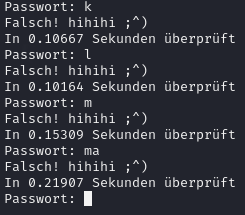
\includegraphics[width=0.35\textwidth]{./imgs/newton_img/NewtonUndCoKG_0.png}
		}
		\caption{Antworten des Servers}
		\label{fig:newton1}
	\end{figure}

	Dabei ist mir folgendes aufgefallen:
	\begin{itemize}
		\item Bei einem falschen Zeichen benötigt die Überprüfung ungefähr 0.1 Sekunden
		\item Beim richtigen Zeichen dauert es ca. 0.05 Sekunden länger
		\item Pro korrekter Stelle steigt die Zeit um etwa 0.1 Sekunden
	\end{itemize}
	Mit diesem gewonnenen Wissen, entschied ich mich dazu, ein Python-Skript zu schreiben:

	\lstinputlisting[caption=TimingBruteforce.py,label=code:newton,style=simple]{TimingBruteforce.py}

	Bevor ich dieses ausführen konnte, musste ich zuerst das Port-Forwarding einrichten: \\
	\lstinline{ssh -L 9999:10.10.10.202:7044 lab} \\
	Das Skript benutzt die \lstinline{socket} Bibliothek, um mit dem Server zu kommunizieren. Nach Start des Skripts, wird die Verbindung zum Server über den weitergeleiteten Port hergestellt.
	Anschließend wird das Teampasswort an den Server geschickt. Daraufhin beginnt das Cracken des Passworts. Stelle für Stelle werden alle möglichen Zeichen durchprobiert, wobei die vom Server retournierte Zeit gespeichert wird.
	Es wird das Zeichen gewählt, bei dem die Überprüfungsdauer am längsten ist.
	Nach 20 Zeichen und etlicher Zeit war das Passwort gecrackt:

	\begin{figure}[h!]
		\centering
		\fbox{
		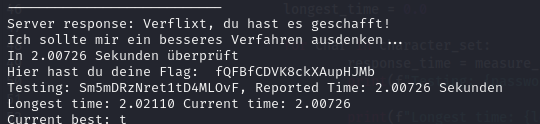
\includegraphics[width=0.9\textwidth]{./imgs/newton_img/NewtonUndCoKG.png}
		}
		\caption{Flag gefunden}
		\label{fig:newton2}
	\end{figure}

	\newpage
	

	\section{Antike Mobile Security}

	\subsection{iTimeTravel}
	Bei dieser Aufgabe wurden iOS-Anwendungsdaten aus verschiedenen lokalen Speichern
	analysiert. Die folgenden Speicherorte wurden untersucht:

	\begin{itemize}
		\item NSUserDefaults in:
			\begin{itemize}
				\item \lstinline{Application/314A301E-B0C5-4698-A396-7CA896D7B486/Documents/userinfo.plist}:
					\begin{itemize}
						\item Name: Manzana

						\item Telefonnummer: 004367705619025

						\item Status: ''Hi, I'm using SupChat!''
					\end{itemize}

				\item \lstinline{Application/992CB749-C531-4E83-9F43-9FA66CDFD68D/Library/Preferences/com.healthapp.health.plist}:
					\begin{itemize}
						\item Name: Manzana

						\item SVNR: 1234 010490

						\item PIN: 6210
					\end{itemize}
			\end{itemize}
			.plist Dateien wurden simpel mit Xcode geöffnet und mit dem eingebauten XML
			Viewer ausgelesen.

		\item CoreData in \lstinline{Application/5FAD1E78-32D1-4C5F-929D-FD098D4AF4D4/Library/Application\ Support/Data.sqlite}:
			\begin{itemize}
				\item Heimatadresse: Favoritenstraße 9, 1040 Wien

				\item Arbeitsadresse: Operngasse 21, 1040 Wien

				\item Weltcafe-Standort: Schwarzspanierstraße 15, 1090 Wien

				\item IoT-Gerätekonfigurationen für Lampen und Staubsaugerroboter
			\end{itemize}

			.sqlite Dateien wurden mit dem ''DB Browser for SQLite'' geöffnet und dort
			im ''Browse Data'' Tab ausgelesen.

		\item Cache-Daten in \lstinline{Application/AA9D9B8E-6B1E-4291-B8D1-CDC808498916/Library/Caches/net.medx.Ada.production/Cache.db}:
			\begin{itemize}
				\item IP-Adresse: 84.115.235.203

				\item Standortdaten: Wien

				\item Gesundheits-API Calls
			\end{itemize}

			.db Dateien wurden ebenfalls mit dem ''DB Browser for SQLite'' geöffnet
			und dort im ''Browse Data'' Tab ausgelesen.

		\item Screenshot-Cache:
			\begin{itemize}
				\item Bankdaten in \lstinline{Application/0420C351-0FF4-47C9-82A6-46453BE6ABAA/Library/SplashBoard/Snapshots/sceneID_com.apple.mobilenotes-83EBA897-8A74-4960-B47A-784C165CA77C/082886CC-F8CE-4C60-B146-E42268573330@2x.ktx}
					\begin{itemize}
						\item IBAN: AT02 1200 0007 0344 7144

						\item BIC: BKAUATWW

						\item Kreditkarte: 2222 4000 7000 0005 (Ablauf: 03/30, CVC: 737)

						\item Bank-PIN: 9RkX4a87mF
					\end{itemize}

				\item Versicherungsinformationen in \lstinline{Application/0A1A5639-A370-4CBC-8194-3BF58CBE5A8C/Library/SplashBoard/Snapshots/sceneID_at.privateversicherung.app-default/A672ACD7-891C-4C45-BDF2-B3FDF5B42381@2x.ktx}
					\begin{itemize}
						\item Versicherungsnummer: 500/1234567-8

						\item Monatliche Prämie: €100,00

						\item Startdatum: 01.01.2015
					\end{itemize}
			\end{itemize}
	\end{itemize}

	.ktx Dateien waren am einfachsten auszulesen, da auf MacOS diese mit dem Apple
	Previewer lesbar sind, so wurden aus diesen die Infromationen ausgelsen.

	\textbf{Profil der Person:}
	\begin{itemize}
		\item Name: Manzana

		\item Telefonnummer: 004367705619025

		\item Geburtsdatum: 01.04.1990

		\item Wohnadresse: Favoritenstraße 9, 1040 Wien

		\item Arbeitsadresse: Operngasse 21, 1040 Wien

		\item Häufiger Aufenthaltsort: Weltcafe, Schwarzspanierstraße 15, 1090 Wien

		\item Versicherungsnummer: 500/1234567-8 (seit 01.01.2015, monatliche Prämie
			€100)

		\item Bankverbindung:
			\begin{itemize}
				\item IBAN: AT02 1200 0007 0344 7144

				\item BIC: BKAUATWW

				\item Kreditkarte: 2222 4000 7000 0005 (gültig bis 03/30)
			\end{itemize}

		\item Smart Home Geräte:
			\begin{itemize}
				\item Diverse IoT-Lampen

				\item Staubsaugroboter
			\end{itemize}

		\item Gesundheitsdaten:
			\begin{itemize}
				\item Verschiedene Symptome und Krankheitsbilder
			\end{itemize}

		\item Technische Daten:
			\begin{itemize}
				\item IP-Adresse: 84.115.235.203

				\item Häufiger Aufenthaltsort laut Standortdaten: Wien
			\end{itemize}
	\end{itemize}

	\subsection{AND(roid)ERS}
	Nicht gelöst.

	\section{Babycam Espionage}

	\subsection{The Rise of the HuManoiD5}
	Nicht gelöst.

	\subsection{ETA}
	Nicht gelöst.

	\section{Das Social Media der Zukunft}

	\subsection{Der vergiftete Passwort Reset}
	Nicht gelöst.

	\subsection{Accountübernahme}
	Nicht gelöst.

	\section{Hidden Timelines}

	\subsection{Phantom Domain}
	Nicht gelöst.

	\section{Vault Voyage}

	\subsection{That's all your vault!}
	Nicht gelöst.

	\section{Wikinger Overflow}

	\subsection{\"Uberlauf. Hand drauf.}
	Nicht gelöst.

	\subsection{Typisch Typing ... Stufe 1}
	Nicht gelöst.

	\subsection{Typisch Typing ... Stufe 2}
	Nicht gelöst.

	\subsection{Typisch Typing ... Stufe 3}
	Nicht gelöst.

	\section{Tap to the Future}

	\subsection{Tick Tock Tap}
	Nicht gelöst.

	\section{So viele}

	\subsection{Das Device ist heiß}
	Nicht gelöst.

	\subsection{Persona non grata}
	Nicht gelöst.

	\subsection{Eine Frage der Kommunikation}
	Nicht gelöst.

	\subsection{Treffpunkt}
	Nicht gelöst.

	\subsection{Alles dokumentiert!}
	Nicht gelöst.

	\subsection{Es geht immer um Inhalte}
	Nicht gelöst.

	\section{Web of Treats}
	Nicht gelöst.

	\subsection{Mitgliedschaftsnr.}
	Nicht gelöst.

	\subsection{Geheimer Artikel}
	Nicht gelöst.

	\subsection{\"Uberf\"ullt}
	Nicht gelöst.

	\subsection{A shell in the forest?}
	Nicht gelöst.

	\subsection{Elvis}
	Nicht gelöst.

	\section{Das. Beste. Text. Adventure. Aller. Zeiten.}

	\subsection{Time to travel!}
	Nicht gelöst.

	\subsection{Mein Name?}
	Nicht gelöst.

	\subsection{Ein PIN!}
	Nicht gelöst.

	\subsection{Ach ... ein Schl\"ussel}
	Nicht gelöst.

	\subsection{Flag!}
	Nicht gelöst.

	\section{Passwörter werden wir auch nie los, oder?!}

	\subsection{Gute Idee, um ein Passwort zu verstecken?!}
	Nicht gelöst.

	\subsection{Call Julius ... äh. John.}
	Nicht gelöst.

	\subsection{Nicht nur Ziffern, sonder auch ...?}
	Nicht gelöst.

	\subsection{/etc/ANTIK?}
	Nicht gelöst.

	\subsection{Sicher sicher?}
	Nicht gelöst.

	\subsection{Zeitlose Liste}
	Nicht gelöst.

	\subsection{(Image)magic(k)}
	Nicht gelöst.

	\subsection{Auch in Zukunft ein schweres Passwort?}
	Nicht gelöst.

	\section{Franz Joseph und die Kommandozeile}

	\subsection{Stage}
	Bei diesem Beispiel musste man sich mit dem Befehl \lstinline{ssh e12122544@tese.esse-teaching.at -p 12345}
	in tese einloggen und von dort mit dem Befehl \lstinline{ssh eisec_team44@10.10.10.201 -p 22044}
	zum vorgebenen Host verbinden. Hier gab es eine ''welcome.txt'' Datei welche Beschrieb
	dass ich mich in den user stage00 einloggen soll und dort die Aufgabe machen soll.
	Die Aufgabe war es einen username mit verstecktem Passwort zu finden. Für diese
	Stage haben mich die folgenden Schritte zum Ziel geführt.

	Nach dem verbinden zur vorgegebenen Maschine:
	\begin{itemize}
		\item Ausführen von \lstinline{ls -la}

		\item Interessanten versteckten Ordner gefunden

		\item In den Ordner gewechselt mit \lstinline{cd}

		\item Erneut \lstinline{ls -la} ausgeführt

		\item Interessante versteckte Datei gefunden

		\item Inhalt der Datei ausgegeben

		\item Fertig
	\end{itemize}

	Lösung:
	\begin{itemize}
		\item Username: stage01

		\item Passwort: bi0owaiK6ieK
	\end{itemize}
	Das folgende Bild zeigt die ausgeführten Befehle in der Kommandozeile.
	\begin{figure}[h!]
		\centering
		\fbox{
		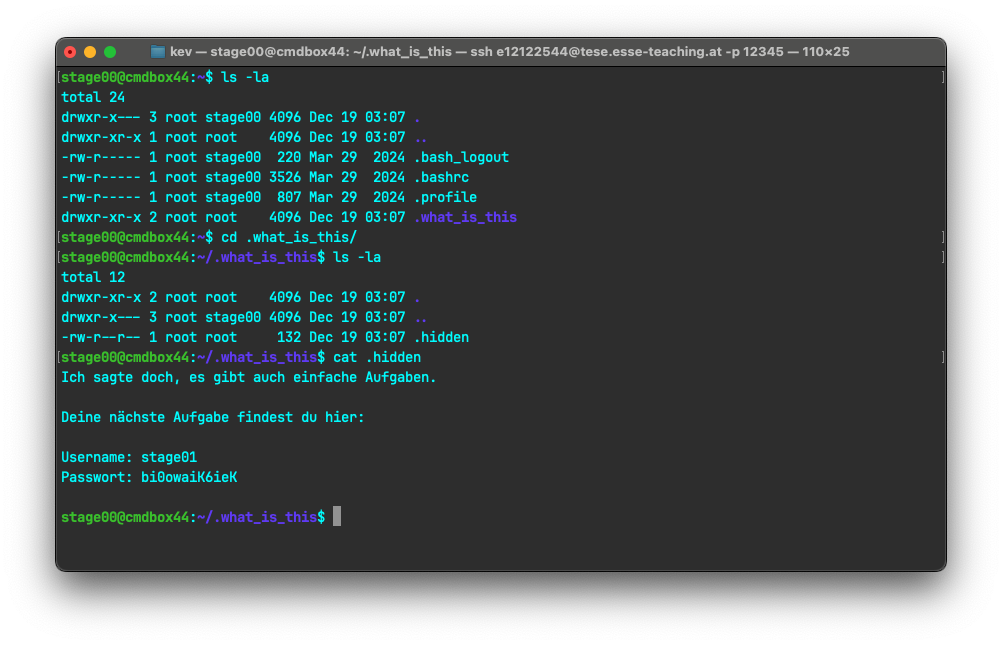
\includegraphics[width=0.8\textwidth]{imgs/stage_img/stage_solution.png}
		}
		\caption{Lösungsweg ''Stage''}
		\label{fig:stage_solution}
	\end{figure}

	\subsection{Stagee}
	Dieses Beispiel hatte dieselbe Aufgabe wie die vorige, undzwar ein verstecktes
	Passwort finden. Hier war ich schon auf der richtigen Maschine eingeloggt, ich
	musste nurmehr user wechseln welchen ich aus der vorigen Ausgabe erhalten habe.
	Für diese Stagee haben mich die folgenden Schritte zum Ziel geführt:

	\begin{itemize}
		\item Einloggen mit dem gegebenen Benutzer: \lstinline{su -l stage01}

		\item Ausführen von \lstinline{ls -la}

		\item Interessante Datei \lstinline{.dump} gefunden, die in ''Stage'' nicht vorhanden
			war

		\item Dateiinhalt mit \lstinline{cat .dump} ausgegeben

		\item Die Hexadezimaldaten mit einem Hex-Decoder decodiert

		\item Fertig
	\end{itemize}

	Lösung:
	\begin{itemize}
		\item Username: stage02

		\item Passwort: othie9chai8V
	\end{itemize}

	Das folgende Bild zeigt die ausgeführten Befehle in der Kommandozeile.
	\begin{figure}[h!]
		\centering
		\fbox{
		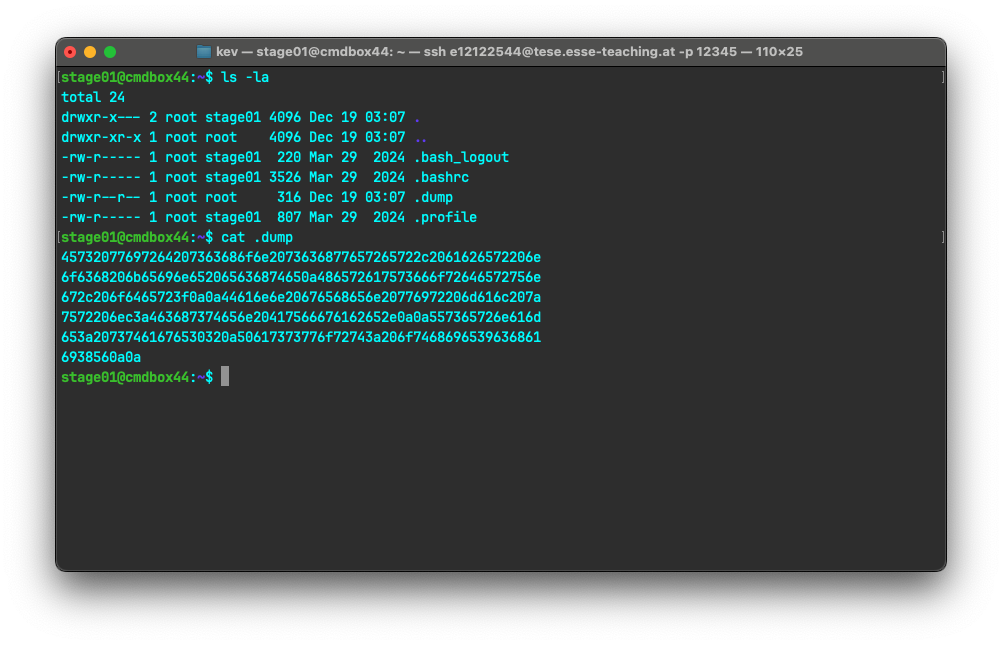
\includegraphics[width=0.8\textwidth]{imgs/stage_img/stagee_solution.png}
		}
		\caption{Lösungsweg ''Stagee''}
		\label{fig:stagee_solution}
	\end{figure}

	\subsection{Stageee}
	Bei diesem Beispiel war es wieder dasselbe. Für diese Stageee haben mich die
	folgenden Schritte zum Ziel geführt:

	\begin{itemize}
		\item Einloggen mit dem gegebenen Benutzer: \lstinline{su -l stage02}

		\item Ausführen von \lstinline{ls -la}

		\item Interessante \lstinline{.compressed.gz} Datei gefunden

		\item Konnte sie nicht mit \lstinline{gunzip} entpacken, daher Inhalt mit \lstinline{zcat}
			ausgelesen

		\item Inhalt wird ausgegeben

		\item Fertig
	\end{itemize}

	Lösung:
	\begin{itemize}
		\item Username: stage03

		\item Passwort: aeteet1iMa2o
	\end{itemize}

	Das folgende Bild zeigt die ausgeführten Befehle in der Kommandozeile.
	\begin{figure}[h!]
		\centering
		\fbox{
		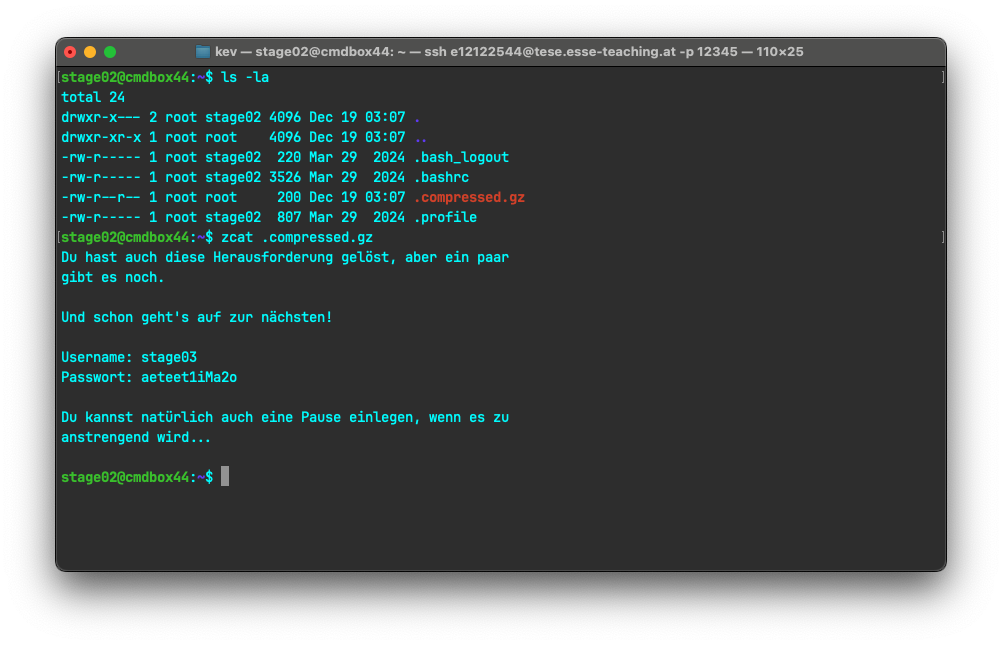
\includegraphics[width=0.8\textwidth]{imgs/stage_img/stageee_solution.png}
		}
		\caption{Lösungsweg ''Stageee''}
		\label{fig:stageee_solution}
	\end{figure}

	\subsection{Stageeee}
	Bei diesem Beispiel war es wieder dasselbe. Für diese Stageee haben mich die
	folgenden Schritte zum Ziel geführt:

	\begin{itemize}
		\item Einloggen mit dem gegebenen Benutzer: \lstinline{su -l stage03}

		\item Ausführen von \lstinline{ls -la}

		\item Interessante \lstinline{.compressed.unknown.rar} Datei gefunden

		\item \lstinline{zcat} auf die Datei ausgeführt

		\item Inhalt wird ausgegeben

		\item Fertig
	\end{itemize}

	Lösung:
	\begin{itemize}
		\item Username: stage04

		\item Passwort: BooR7nie1chu
	\end{itemize}

	Das folgende Bild zeigt die ausgeführten Befehle in der Kommandozeile.
	\begin{figure}[h!]
		\centering
		\fbox{
		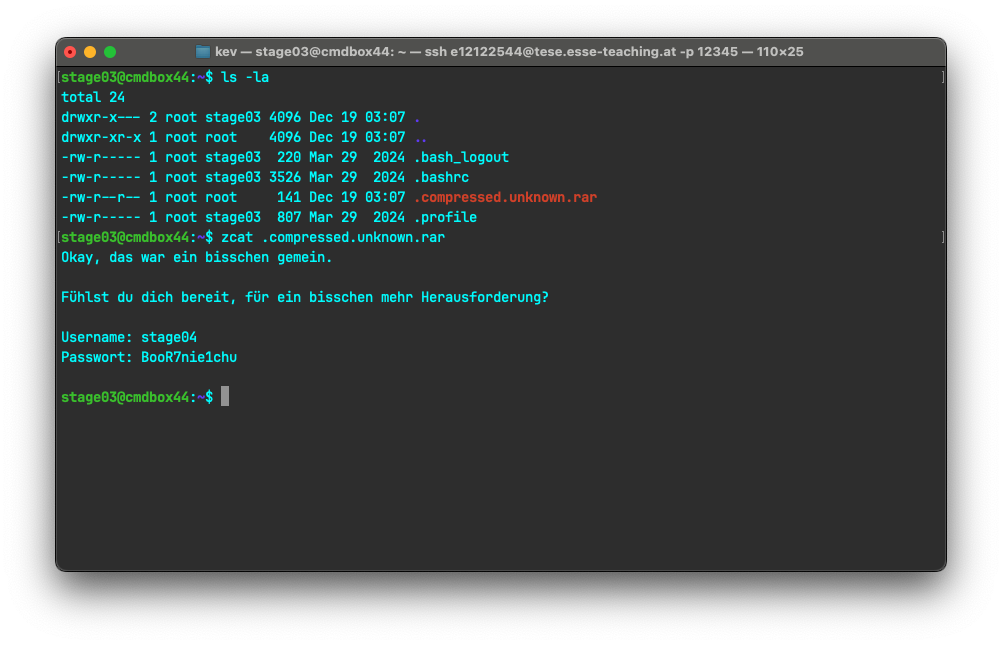
\includegraphics[width=0.8\textwidth]{imgs/stage_img/stageeee_solution.png}
		}
		\caption{Lösungsweg ''Stageeee''}
		\label{fig:stageeee_solution}
	\end{figure}

	\subsection{Stageeeee}
	Bei diesem Beispiel war es wieder dasselbe. Für diese Stageee haben mich die
	folgenden Schritte zum Ziel geführt:

	\begin{itemize}
		\item Einloggen mit dem gegebenen Benutzer: \lstinline{su -l stage04}

		\item Ausführen von \lstinline{ls -la}

		\item Interessante \lstinline{.encrypted} Datei gefunden

		\item \lstinline{cat} auf die Datei ausgeführt, um den Inhalt auszugeben

		\item Inhalt scheint verschlüsselt zu sein

		\item Sieht nach Base64 aus

		\item In Base64-Decoder eingegeben (Ausgabe siehe
			\ref{fig:stageeeee_base64_output})

		\item Zufällige Zeichen deuten darauf hin, dass es komprimiert sein könnte

		\item Mit Base64-Befehl entschlüsselt, entpackt und direkt auf die
			Konsolenausgabe ausgegeben, da das Schreiben in Dateien in diesem Verzeichnis
			nicht erlaubt ist. Folgender Befehl wurde verwendet: \lstinline{base64 -d .encrypted | gunzip}

		\item Fertig
	\end{itemize}

	Lösung:
	\begin{itemize}
		\item Username: stage05

		\item Passwort: eifietiey2Go
	\end{itemize}

	\begin{figure}[h!]
		\centering
		\fbox{
		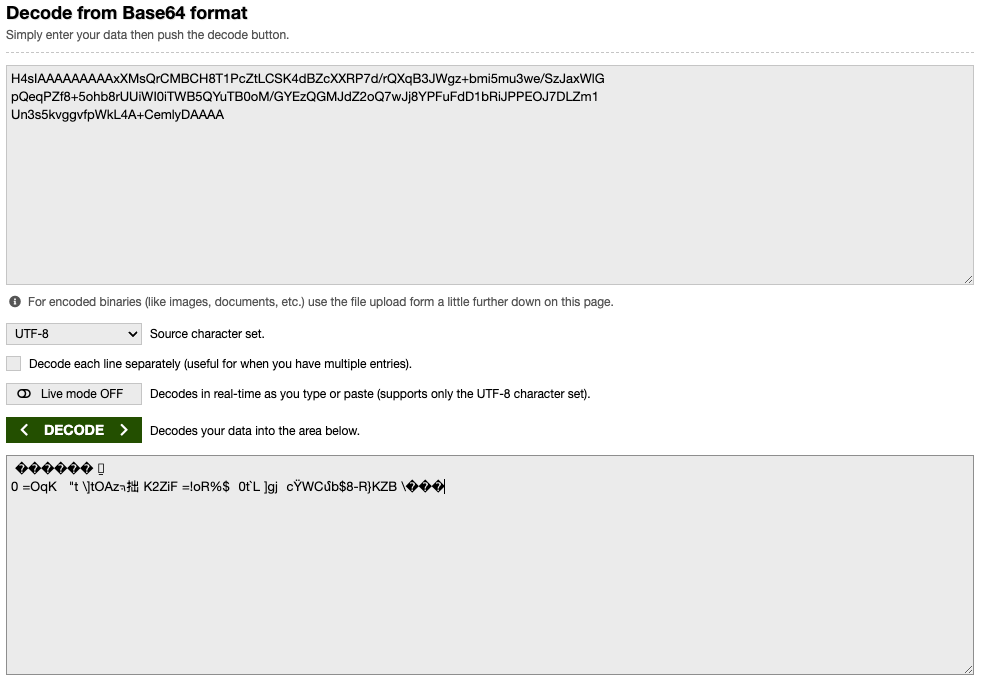
\includegraphics[width=0.8\textwidth]{
			imgs/stage_img/stageeeee_base64_output.png
		}
		}
		\caption{Ergebnis der base64 Dekodierung von dem Inhalt der Datei .encrypted}
		\label{fig:stageeeee_base64_output}
	\end{figure}

	\begin{figure}[h!]
		\centering
		\fbox{
		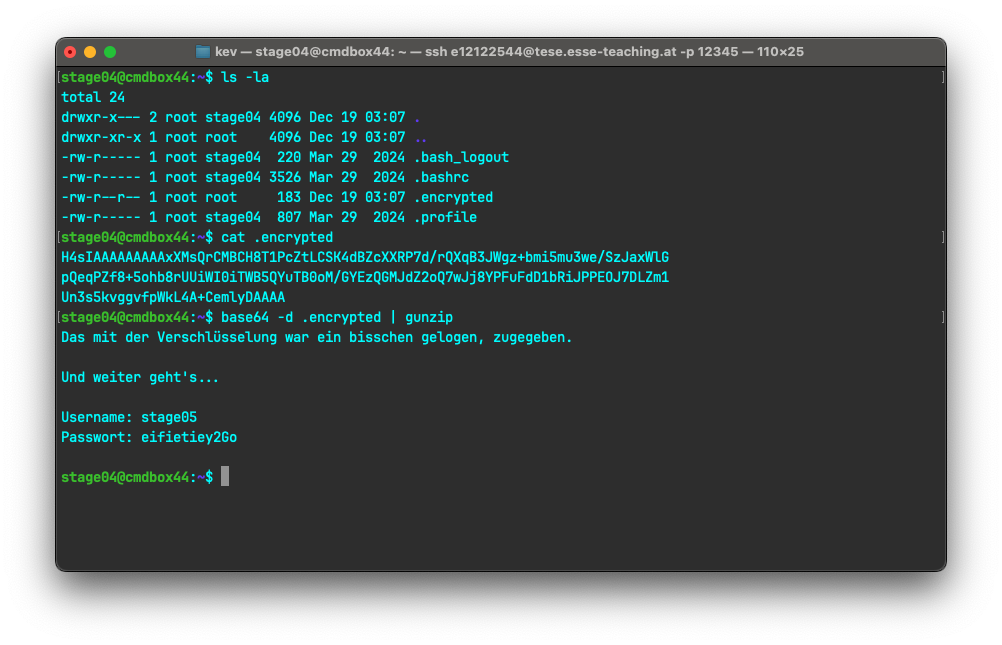
\includegraphics[width=0.8\textwidth]{imgs/stage_img/stageeeee_solution.png}
		}
		\caption{Lösungsweg ''Stageeeee''}
		\label{fig:stageeeee_solution}
	\end{figure}

	\newpage

	\subsection{Stageeeeee}
	Nicht gelöst.

	\subsection{Stageeeeeee}
	Nicht gelöst.

	\subsection{Stageeeeeeee}
	Nicht gelöst.

	\subsection{Stageeeeeeeee}
	Nicht gelöst.

	\subsection{Stageeeeeeeeee}
	Nicht gelöst.

	\subsection{Stageeeeeeeeeee}
	Nicht gelöst.

	\subsection{Stageeeeeeeeeeee}
	Nicht gelöst.

	\section{Ueberschrift 1}

	\subsection{Hinweise}
	\emph{Hinweise:}
	\begin{itemize}
		\item Verwenden Sie entweder diese deutsche Version oder die englische Version
			in \lstinline{protocol.tex}.

		\item Setzen Sie alle Variablen nach \emph{FOR STUDENTS} in der .tex Datei.

		\item Ersetzen Sie die Platzhalter für Ihre Namen und MatNr.

		\item Löschen Sie diese Sektion über Hinweise und die folgenden Beispiel-Kapitel.

		\item Achten Sie auf geforderte Formate und Anforderungen an die Dateinamen.

		\item Führen Sie \lstinline{pdflatex} mindestens zweimal aus, damit die Referenzen
			und Seitenzahlen richtig im PDF dargestellt werden.

		\item Sie können dazu auch das Makefile verwenden: \lstinline{make de}.
	\end{itemize}

	\section{Beispiele}

	\subsection{Source Code formatieren}
	Es folgen einige Beispiele wie Sourcecode in diesem Dokument formatiert und
	referenziert werden kann (\hyperref[code:beispiel1]{siehe Listing~\ref*{code:beispiel1}
	auf Seite~\pageref*{code:beispiel1}} und \hyperref[code:beispiel2]{siehe
	Listing~\ref*{code:beispiel2} auf Seite~\pageref*{code:beispiel2}}).

	Ebenso können kurzer Code oder kurze Befehle direkt in der Zeile in einem
	\lstinline{lstinline Block} mit typengleicher Schrift formatiert werden.

	\lstinputlisting[caption=Example C/C++ file,label=code:beispiel1,style=c]{example.c}

	\begin{lstlisting}[caption=Example bash script,label=code:beispiel2,style=simple]
#!/bin/bash
echo "Bash version ${BASH_VERSION}..."
for i in {0..10..2}
  do
     echo "Welcome $i times"
 done

echo "some very very very very very very very very very very very very very very very very very very very very long string"

exit 0;
\end{lstlisting}

	\subsection{Bilder}

	Es folgen einige Beispiele wie Bilder in diesem Dokument eingefuegt werden
	koennen (\hyperref[fig:logo1]{siehe Abbildung~\ref*{fig:logo1} auf Seite~\pageref*{fig:logo1}}).

	\begin{figure}[h!]
		\centering
		\fbox{
		
\includegraphics[width=0.4\textwidth]{./imgs/logos/esse-logo-color.png}
		}
		\caption{ESSE Logo}
		\label{fig:logo1}
	\end{figure}

	%%%%%%%%%%%%%%%%%%%%%%%%%%%%%%%%%%%%%%%%%%%%%%%%%%%%%%%%%%%%%%%%%%%%%%
	%
	% DO NOT CHANGE THE FOLLOWING PART
	%
	%%%%%%%%%%%%%%%%%%%%%%%%%%%%%%%%%%%%%%%%%%%%%%%%%%%%%%%%%%%%%%%%%%%%%%
\end{document}